\documentclass[11pt,a4paper]{article}
\usepackage[margin=2.5cm]{geometry}
\usepackage{cmap}
\usepackage[T1]{fontenc}
\usepackage{lmodern}
\usepackage{amsmath,amssymb,booktabs,graphicx,tabularx,array}
\usepackage[authoryear,round]{natbib}
\usepackage{xurl}
\usepackage{needspace}
\usepackage[colorlinks=true,linkcolor=blue,citecolor=blue,urlcolor=blue]{hyperref}
\graphicspath{{figures/}{paper_support/results/}{paper_support/inherited_F10/results/}}
\newcommand{\SIref}[1]{\csname SIlabel:#1\endcsname}
\expandafter\def\csname SIlabel:fig:SI_Indonesia\endcsname{S2}
\expandafter\def\csname SIlabel:fig:SI_coverage\endcsname{S1}
\expandafter\def\csname SIlabel:tab:SI_Canada_components\endcsname{S24}
\expandafter\def\csname SIlabel:tab:SI_FIN_stock_flow\endcsname{S23}
\expandafter\def\csname SIlabel:tab:SI_France_contrasts\endcsname{S25}
\expandafter\def\csname SIlabel:tab:SI_France_windows\endcsname{S22}
\expandafter\def\csname SIlabel:tab:SI_Indonesia_classes\endcsname{S17}
\expandafter\def\csname SIlabel:tab:SI_account_sensitivity\endcsname{S2}
\expandafter\def\csname SIlabel:tab:SI_account_sensitivity_2010_2020\endcsname{S3}
\expandafter\def\csname SIlabel:tab:SI_account_sensitivity_2015_2022\endcsname{S4}
\expandafter\def\csname SIlabel:tab:SI_class_support\endcsname{S16}
\expandafter\def\csname SIlabel:tab:SI_component_contributions\endcsname{S5}
\expandafter\def\csname SIlabel:tab:SI_conversion_exact\endcsname{S20}
\expandafter\def\csname SIlabel:tab:SI_forest_decomposition\endcsname{S6}
\expandafter\def\csname SIlabel:tab:SI_inventory_cells\endcsname{S21}
\expandafter\def\csname SIlabel:tab:SI_regional_compensation\endcsname{S19}
\expandafter\def\csname SIlabel:tab:SI_transition_events\endcsname{S18}
\expandafter\def\csname SIlabel:tab:brazil_cover\endcsname{S12}
\expandafter\def\csname SIlabel:tab:contrast\endcsname{S14}
\expandafter\def\csname SIlabel:tab:countries\endcsname{S1}
\expandafter\def\csname SIlabel:tab:domain\endcsname{S9}
\expandafter\def\csname SIlabel:tab:frontier\endcsname{S15}
\expandafter\def\csname SIlabel:tab:native_sd\endcsname{S11}
\expandafter\def\csname SIlabel:tab:nativecoverage\endcsname{S10}
\expandafter\def\csname SIlabel:tab:products\endcsname{S7}
\expandafter\def\csname SIlabel:tab:quality\endcsname{S8}
\expandafter\def\csname SIlabel:tab:reference_coverage\endcsname{S13}

\newcommand{\NationalRows}{13652}
\newcommand{\CountryIDs}{236}
\newcommand{\AccountPass}{183}
\newcommand{\AccountFail}{53}
\newcommand{\PilotPass}{8}

\newcommand{\MapNet}{65.24}
\newcommand{\MapGain}{142.21}
\newcommand{\MapLoss}{76.97}
\newcommand{\MapCancellation}{70.23}
\newcommand{\WholeWidth}{993.09}
\newcommand{\ReductionForm}{49.05}
\newcommand{\RatioForm}{1.4555}
\newcommand{\ReductionSav}{55.93}
\newcommand{\RatioSav}{1.9495}

\emergencystretch=3em
\renewcommand{\topfraction}{0.9}
\renewcommand{\textfraction}{0.07}
\renewcommand{\floatpagefraction}{0.85}
\setcounter{topnumber}{3}
\title{Ecological assets behind improving accounts:\\national forest evidence and biomass-change identifiability}
\author{Amin Abaee\\\small Independent Researcher, Tehran, Iran\\\small\href{mailto:amin_abaee@ut.ac.ir}{amin\_abaee@ut.ac.ir}\\\small ORCID: \href{https://orcid.org/0000-0002-0019-1842}{0000-0002-0019-1842}}
\date{}
\hypersetup{pdftitle={Ecological assets behind improving accounts: national forest evidence and biomass-change identifiability},pdfauthor={Amin Abaee},pdfkeywords={Ecological Footprint; Biocapacity; Natural capital accounting; Above-ground biomass; Partial identification; Subpixel biomass allocation; Land-use change}}
\begin{document}
\maketitle
\begin{abstract}
Increasing productivity-weighted accounts need not identify ecological asset gains. We combine national account trajectories, source-specific mapped forest series, official inventory evidence and a boundary-matched biomass identification experiment. Of 183 eligible account identifiers in 2015--2023, 91 increase in total biocapacity; 68 of these have a decreasing forest account component, an accounting result rather than independent forest-loss evidence. Published mapped groups decline by 10.863, 0.703 and 3.303 million ha in Brazil, Indonesia and the Democratic Republic of the Congo, respectively, without calibrated change intervals. Annual transition constraints bound the Indonesian 2015-forest-to-2023-oil-palm cohort at 0.112--2.326 million ha, conditional on classifications, without equating repeated events with unique hectares. Official inventories yield conditional positive volume differences for Finnish and French campaign windows without assuming cross-inventory independence; Canada's earlier inventory-domain AGB change interval includes zero and its uncertainty representations require reconciliation. On the fixed 61,830 ha Brazilian footprint, the auxiliary whole-cell biomass point-map total increases by $\MapNet\times10^3$ Mg, while $\MapCancellation\%$ of absolute local differences cancels. Constructive allocations preserve every cell total and mapped fraction yet permit all four joint sign quadrants for nested cover groups. Native-cell mass information narrows identification sets by $\ReductionForm\%$ and $\ReductionSav\%$ relative to one-window totals but identifies neither sign; density-contrast restrictions identify sensitivity thresholds, not established ecological facts. None of eight candidates supplies the original calibrated national 2015--2023 forest-AGB comparison. The results establish national evidence and increments of identification while distinguishing mapped extent, inventory volume, biomass and uncertainty. They do not establish national ecological composition masking, conversion associations or independent reporting accuracy.
\end{abstract}

\noindent\textbf{Keywords:} Ecological Footprint; Biocapacity; Natural capital accounting; Above-ground biomass; Partial identification; Subpixel biomass allocation; Land-use change.


\section{Introduction}
Biocapacity is expressed in global hectares, combining physical area with productivity-based factors. Above-ground biomass is a mass of specified living woody material within a geographic support. These quantities are related through ecological production but are not interchangeable measures of ecosystem assets. The distinction between natural-capital stocks and accounting flows has an established basis in the Ecological Footprint literature \citep{Mancini2017}. A quantitative assessment requires separate observation operators and an explicit treatment of their domains.

Composition-dependent land-use models show that transfers towards a land class with a higher annual contribution per hectare can increase a model account while reducing another land class's area \citep{Abaee2026}. Such a mechanism motivates an empirical comparison but does not determine the sign of an observed forest-stock trend. Existing European forest-condition accounting also demonstrates the importance of spatially heterogeneous changes within an aggregate \citep{Maes2023}. Forest condition, extent, biomass and regeneration remain distinct ecological attributes.

\Needspace{15\baselineskip}
The ecological hypothesis motivates five linked measurement questions:
\begin{enumerate}
\item What national account trajectories and component sensitivities are observed, and how do they differ from source-specific physical forest quantities?
\item Within a matched local footprint, can an increasing whole-cell biomass point-map total rule out a decline in a separately defined mapped-cover group?
\item How do spatial aggregation, native-cell mass information and explicit density-contrast restrictions change group-change identification sets?
\item What unique endpoint cohorts are constrained by annual national class-transition tables, without treating repeated events as unique converted area?
\item What stock-change statements do official inventory designs and defensible dependence or bias bounds support on their actual periods and domains?
\end{enumerate}
The first question is answered by the national trajectories and typed source comparisons (Section~\ref{sec:nationalresults}); the second and third by constructive allocation, joint sets and information sensitivities; the fourth by the marked-flow bounds (Section~\ref{sec:flowresults}); and the fifth by the inventory results (Section~\ref{sec:inventoryresults}). The original calibrated national 2015--2023 forest-AGB target is retained separately. Neither nominal mapped discordance nor conditional inventory-volume change substitutes for it. Exact paired field censuses and known covariance are not imposed as universal prerequisites: compatible marginal inventory designs, direct change estimates or defensible dependence and bias bounds can also support an inference.

\section{Materials and methods}
\subsection{Accounts, physical quantities and comparison domains}
The National Ecological Footprint and Biocapacity Accounts, Edition 2026, results and metadata v1.0, supply annual biocapacity in global hectares (gha) \citep{Lo2026}. We require complete 2015--2023 records, admissible publication flags, finite nonnegative components, positive population and component-sum consistency. Of 236 country/territory identifiers, 183 satisfy these account criteria; physical-data eligibility is assessed separately (Supplementary Figure~\SIref{fig:SI_coverage} and Table~\SIref{tab:countries}). We calculate endpoint changes, all five component contributions, exclusions of fishing and built land, and separately labelled per-person changes. The 2010--2020 account sensitivity includes 182 members of the primary cohort; the additional 2015--2022 sensitivity does not supersede it. Primary and secondary domain values appear in Supplementary Tables~\SIref{tab:SI_account_sensitivity}, \SIref{tab:SI_account_sensitivity_2010_2020} and \SIref{tab:SI_account_sensitivity_2015_2022}; all five primary component contributions and the forest-account area-by-factor decomposition appear in Tables~\SIref{tab:SI_component_contributions} and \SIref{tab:SI_forest_decomposition}.

The eight physical candidates are an exploratory logistical set, not a representative or outcome-naive sample. Acquisition continued with account directions and earlier results known. We retain all eight, including concordant, discordant and unexecuted cases. Complete MapBiomas national tables supply source-specific mapped extent for Brazil Collection 11, Indonesia Collection 4.1 and DR Congo Collection 1 \citep{MapBiomas2026,MapBiomasIDN2026,MapBiomasCOD2026}. Brazilian formations comprise classes 3, 5, 6 and 49; the distinct formations-plus-savanna group adds 4 and 7. Indonesian forest comprises 3, 5 and 76; Congolese source forest comprises 3, 4 and 5. Plantations are separate. These groups are not a harmonized forest definition. Leaf classes are summed once; Brazilian and Indonesian annual transition margins are reconciled to extent. Congo's country series is used rather than forcing nonclosing subunit totals into a partition. Source definitions and support sensitivities are documented in Supplementary Figure~\SIref{fig:SI_Indonesia} and Table~\SIref{tab:SI_class_support}.

\subsection{Matched support and conditional biomass allocation}
The geometry-selected Brazilian rectangle contains 65,536 native ESA CCI Biomass v7.0 cells covering 61,830.34 ha. Both biomass and MapBiomas endpoints are 2015 and 2023; the footprint is fixed, not chosen by observed change. Native biomass density refers to a whole pixel, not its forest part \citep{SantoroCartus2026,PUG2026}. WGS84 overlap areas map finer cover fractions to that support; missing support is not renormalized away. Product/quality definitions, boundary screening, native access diagnostics and stored-SD diagnostics are given in Supplementary Tables~\SIref{tab:products}--\SIref{tab:quality} and \SIref{tab:domain}, \SIref{tab:nativecoverage} and \SIref{tab:native_sd}; local cover endpoints are in Table~\SIref{tab:brazil_cover}.

Let $q_{it}=A_i\widehat d_{it}$ denote observed full-cell mass. Knowing a group's area fraction does not allocate $q_{it}$ within a mixed cell. Holding point maps and cover exact, we allow nonnegative component masses without finite density caps or temporal coupling. Cells entirely in group $g$ anchor its lower mass bound; every cell intersecting $g$ contributes to its upper bound:
\begin{equation}
\widehat{\mathcal I}_t^g=\left[\sum_{i\in P_t^g}q_{it},\ \sum_{i\in H_t^g}q_{it}\right].\label{eq:allocationmain}
\end{equation}
Endpoint subtraction gives the compatible difference range. All cells, including zeros and mixed/changing cover, remain included. A coherent three-component allocation defines the joint set for formations, added savanna and complement. These are identification sets conditional on observations, not confidence intervals for true forest change.

We compare nested block observations on the identical footprint: coarser blocks preserve mass but remove internal information. Positive and negative local differences quantify arithmetic cancellation, not biological gross turnover. A separate sensitivity bounds the ratio of component densities within each mixed cell by an assumed $R\ge1$; $R=1$ imposes homogeneous allocation and $R\to\infty$ recovers the unrestricted model. No finite $R$ is calibrated here. Observed zeros are retained; zero AGB or stored SD does not certify ecological absence or zero true error. Proofs, reconstructed witnesses, full width comparisons and contrast grids are supplied in the SI, including Tables~\SIref{tab:frontier} and \SIref{tab:contrast}.

\subsection{Endpoint cohorts from annual transition capacities}
Annual transitions count events and may count a hectare repeatedly. We instead mark the land mapped as forest in 2015 and follow its feasible flow through annual class-to-class capacities. Marked flow is bounded by each observed transition and conserved at interior class--year nodes. Minimizing and maximizing its final inflow into a 2023 destination bounds a unique endpoint cohort, allowing intermediate classes. The bounds are sharp for the balanced continuous-area capacity model, not reconstructions of actual histories. We evaluate national and fixed fine-geography networks; geographical restrictions prevent rearrangement across 49 Brazilian units or 38 Indonesian provinces. All 634 saved primal/dual certificates were independently verified. Outward numerical allowances are not classification-error intervals. Supplementary Table~\SIref{tab:SI_conversion_exact} gives all seven fine-geography ranges; the SI provides the model and proof.

For endpoint net-area errors bounded by $e$, change error is bounded by $2e$. Conversion requires a different error control: if initial-forest and final-destination class sets have combined symmetric-difference area at most $E$, a mapped lower cohort bound $L$ transfers only as $\max(0,L-E)$. Small net-area error does not imply small class-set error.

\subsection{Inventory periods, sampling uncertainty and measurement error}
Finnish NFI12 (2014--2018) and NFI13 (2019--2023) supply growing-stock volume and biomass components for productive and poorly productive forest, including \AA land \citep{Korhonen2021,Korhonen2024}. French tables supply living stem volume on metropolitan production forest including Corsica, across four pooled campaign windows \citep{IGN2018,IGN2026}. Inventory-cycle centres are not exact annual endpoints; stem volume is not AGB. Canadian NFI v3.1 supplies earlier-domain AGB stock and annualized change using remeasured 2007--2017 and projected 2006--2017 observations \citep{CanadaNFI2025}.

For approximately normal marginal inventory estimators, Bonferroni endpoint intervals give
\begin{equation}
\Delta\widehat V\ \pm\ z_{0.9875}(s_0+s_1),\qquad z_{0.9875}=2.241403,\label{eq:invbonf}
\end{equation}
with approximate 95\% sampling coverage without assuming cross-inventory independence. We retain a separate Finnish second-moment sensitivity conditional on unbiased errors and reported standard errors representing true error standard deviations; exact coverage is not asserted for estimated variances. For French reported 95\% endpoint halfwidths, direct subtraction guarantees at least 90\% contrast coverage; approximate 95\% rescaling additionally assumes marginal normality. Source rounding is included outward. Neither calculation covers an unbounded differential systematic bias. Canadian provider intervals are retained without inferring precision from the inconsistent RSE representation. Finnish source cells are given in Supplementary Table~\SIref{tab:SI_inventory_cells}; French windows and all contrasts in Tables~\SIref{tab:SI_France_windows} and \SIref{tab:SI_France_contrasts}; Canadian components in Table~\SIref{tab:SI_Canada_components}.

The separate Finnish 2022--2023 forest-account stock--flow reconciliation, including its balancing item, is retained in Supplementary Table~\SIref{tab:SI_FIN_stock_flow}; it is partly inventory-derived and not independent physical validation. Stock validation is not change validation: spatial and temporal dependence, reference error, forest allocation, converted land and differential bias require separate assessment \citep{Olofsson2014,E3UB2025,PVIR2026}. Public local reference artifacts do not supply compatible paired-endpoint validation here; their counts, source compatibility and biomass-reference eligibility are documented in Supplementary Table~\SIref{tab:reference_coverage} and the associated SI protocols. Exact paired censuses and known covariance are not universal prerequisites: compatible designs, direct change estimates and defensible dependence/bias bounds can suffice.

\section{Results}
\subsection{National account trajectories and source-specific forest extent}\label{sec:nationalresults}
Of the 183 eligible account identifiers, total biocapacity increases in 91 and decreases in 92 during 2015--2023. Among increasing totals, the forest account component decreases in 68, increases in 22, and is unresolved at the rounding scale in one. This is account composition, not 68 independently observed forest losses. Figure~\ref{fig:accounts} displays the eight candidate trajectories. Domain choice matters: Canada and Cameroon change total-account direction under some component exclusions. Canada's fishing component contributes $+1.186$ percentage points of its initial total, while its forest component contributes $-0.644$; Cameroon's crop and built components contribute $+1.505$ and $+0.749$, while forest contributes $-1.689$ (Supplementary Table~\SIref{tab:SI_component_contributions}). Within the forest account's own lineage, France combines a $+2.502$ million-gha area contribution with a $-0.655$ factor contribution, whereas Australia combines $+0.339$ with $-0.505$; these are accounting terms, not independent physical area or productivity measurements (Supplementary Table~\SIref{tab:SI_forest_decomposition}). All eight candidates, not only nominally discordant ones, remain in the comparison (Table~\ref{tab:nationalcases}).

\begin{figure}[htbp]
\centering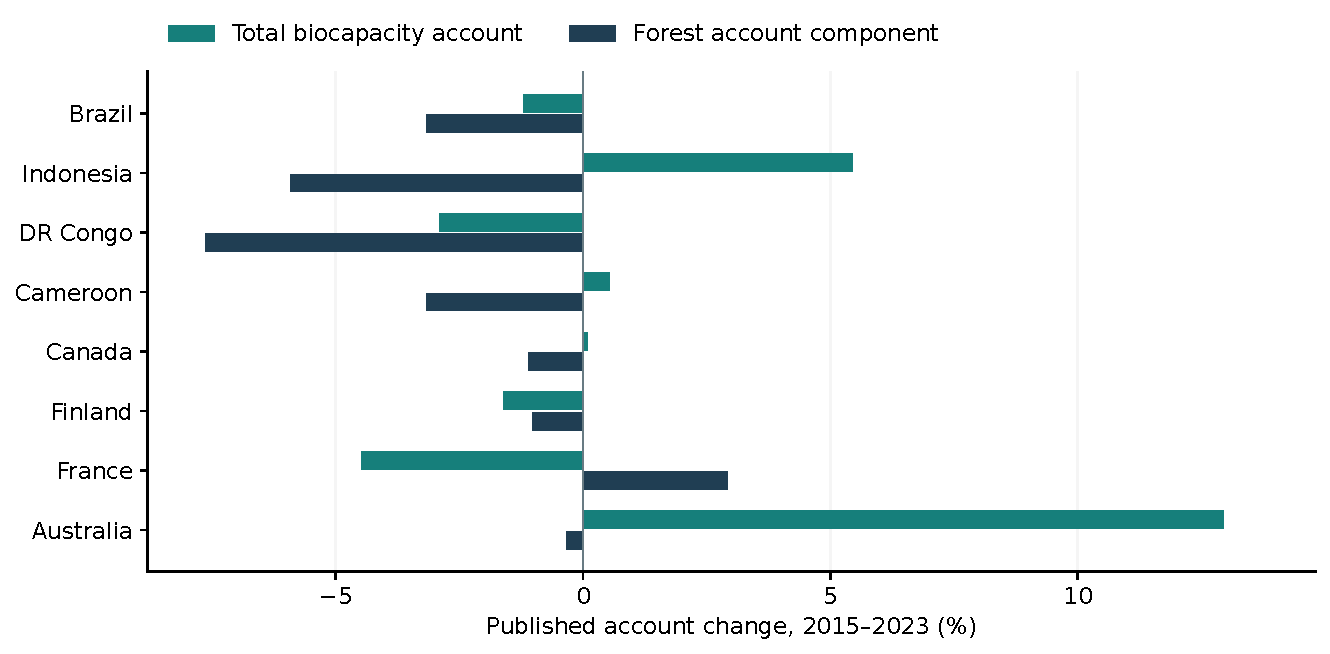
\includegraphics[width=1\textwidth]{account_composition_F15.pdf}
\caption{Account composition across all eight exploratory candidates, 2015--2023. Both series are accounting quantities, not independent observations of ecological stock. Full account-domain and per-person sensitivities appear in Supplementary Table~\SIref{tab:SI_account_sensitivity}. Data: Lo et al. (2026); derived account values retain CC BY-SA 4.0.}\label{fig:accounts}
\end{figure}
\begin{table}[htbp]
\centering\small
\caption{National account changes and separately typed physical evidence. Account columns are percentage changes in gha; mapped extent, volume and biomass are not interchangeable. None completes a calibrated national 2015--2023 forest-AGB comparison. Inventory periods and domains differ.}\label{tab:nationalcases}
\begin{tabularx}{\textwidth}{lp{2.7cm}X}\toprule
Country & Total/forest account (\%) & Physical evidence and qualification\\\midrule
Brazil & $-1.21/-3.15$ & Mapped formations: $-10.863$ Mha ($-2.64\%$), 2015--2023. No calibrated change interval.\\
Indonesia & $+5.46/-5.92$ & Mapped forest: $-0.703$ Mha ($-0.66\%$), 2015--2023. No calibrated change interval.\\
DR Congo & $-2.91/-7.64$ & Source mapped forest: $-3.303$ Mha ($-2.01\%$), 2015--2023. No calibrated change interval.\\
Cameroon & $+0.54/-3.16$ & No completed physical numerical module.\\
Canada & $+0.08/-1.10$ & Earlier inventory-domain AGB: $+17.639$ Mt/year; labelled range $[-21.279,56.557]$. Not 2015--2023.\\
Finland & $-1.60/-1.01$ & Cycle volume: $+76.772$ million m$^3$, 2014--2018 to 2019--2023. Conditional sampling result.\\
France & $-4.47/+2.91$ & Production-forest volume: $+200$ million m$^3$, 2013--2017 to 2021--2025. Method bias not bounded.\\
Australia & $+12.95/-0.33$ & No completed physical numerical module.\\
\bottomrule\end{tabularx}
\end{table}


Brazilian formations decline from 412.016 to 401.154 million mapped ha, a decrease of 10.863 million ha or 2.64\%. The separate formations-plus-savanna group decreases by 18.184 million ha or 3.43\%. Indonesia's source forest decreases from 107.055 to 106.352 million ha, a net decrease of 702,562 ha or 0.66\%, while mapped oil palm increases by 2.833 million ha. Thus Indonesia has a nominal total-account increase and mapped-forest decrease, whereas Brazil has both decreasing. These are not paired calibrated AGB signs, and their two-case pattern is not a reporting-error rate. The combined Indonesian result is definition-sensitive: Forest Formation alone increases by 3,019 ha ($+0.0032\%$), mangrove decreases by 11,620 ha, and peat swamp forest decreases by 693,961 ha ($-6.35\%$). The earlier collection reports a 3.106 million-ha forest decline, but its footprint is 43,130 ha larger. The resulting 2.403 million-ha difference between net changes cannot be attributed solely to version processing. Both collections give a negative combined change, but differ materially in magnitude and support (Supplementary Figure~\SIref{fig:SI_Indonesia} and Table~\SIref{tab:SI_Indonesia_classes}).

Congo's official country table assigns 163.948 and 160.645 million ha to its forest group in 2015 and 2023, a decline of 3.303 million ha or 2.01\%. Dense forest decreases by 1.754 million ha and woodland by 1.577 million ha; mapped mangrove increases by 28,328 ha. Agriculture/pasture increases by 3.098 million ha and plantation by 386,532 ha. The exported country label footprint is approximately 231.405 million ha. Province and biome totals are respectively about 39,860 and 2,516 ha smaller; their net differences are not geometry symmetric differences or proof of a nested missing-area partition. The country series, not a forced subunit sum, supplies the reported result. The ATBD documents class confusion, temporal irregularities and ecotone integration using stable map labels. No compatible reference-based change interval is established, and the agricultural increase is not attributed to forest conversion from marginal totals alone.

For Brazil, Indonesia and Congo, respectively, symmetric endpoint net-area errors would each have to be below approximately 5.431, 0.351 and 1.652 million ha to guarantee the reported negative forest-group difference under that error model. These are requirements on unknown errors, not measured uncertainty budgets. Cover and biomass remain distinct. Spatial netting also matters: 20 of 27 Brazilian states decline and seven increase, with negative and positive state changes summing to $-11.017$ and $+0.155$ million ha; 14 of 38 Indonesian provinces decline and 24 increase, with sums of $-1.303$ and $+0.601$ million ha. These are descriptive mapped compensation patterns, not confidence-resolved losses and gains (Supplementary Table~\SIref{tab:SI_regional_compensation}).

\subsection{A common local support does not identify the forest-group trend}
Figure~\ref{fig:brazil_support} shows the mapped fractions on the matched grid. The fixed footprint has area 61,830.34\,ha and contains $65{,}536$ native biomass cells. Each land-cover subset comprises $846\times845$ finer cells intersecting this rectangle. All target cells have complete published-label coverage at both endpoints under the declared unclassified-code convention. This is classification coverage within the local footprint, not national coverage or evidence that temporal gap filling was unnecessary.

Supplementary Table~\SIref{tab:brazil_cover} distinguishes the mapped quantities. The formations group occupies 6.99\% in 2015 and 7.29\% in 2023; including savannas gives 19.68\% and 18.49\%, respectively. The opposite endpoint directions concern different vegetation groupings and do not establish a resolved ecological change, a preferred forest definition or an account--asset divergence.



There are $13{,}301$ native cells with a nonzero formations fraction at either endpoint and $10{,}385$ at both endpoints, but only $625$ are mapped entirely as formations at both endpoints. Mixed formations cells number $10{,}865$ in 2015 and $11{,}154$ in 2023. These descriptors show the difference between an area fraction and a whole-cell forest selection. Restricting the analysis to persistent pure cells would omit changing and mixed support; that restriction is not used to define a national forest-change sample.

\begin{figure}[htbp]
\centering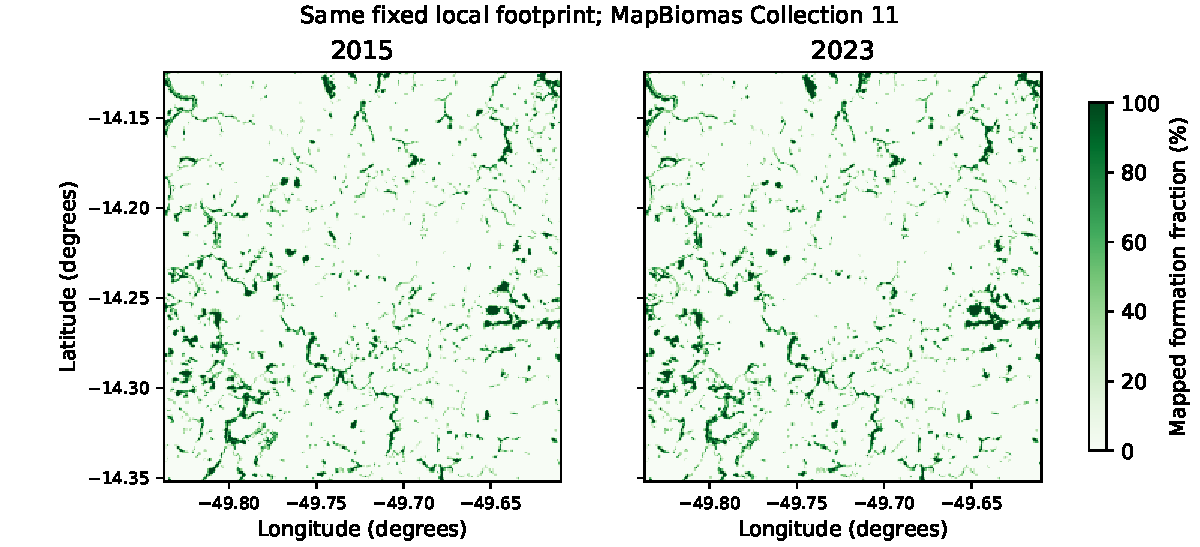
\includegraphics[width=.98\textwidth]{brazil/BRA_F05_support_fractions.pdf}
\caption{Mapped forest-formations fractions within the same fixed local rectangle in 2015 and 2023. Fractions refer to classes 3, 5, 6 and 49; savannas and plantations are separate. The complement includes other vegetation and land uses, not absence of ecological assets. The maps do not estimate biomass change or establish national representativeness. Source: MapBiomas Project, Collection 11; area-overlap processing described in the text.}\label{fig:brazil_support}
\end{figure}

\paragraph{Conditional allocation ranges.}
Table~\ref{tab:allocation} reports the local allocation sets for the same two mapped groups. Both endpoint-difference sets contain zero, permitting negative, zero and positive differences under the minimal allocation model. Thus the sign is not identified by these point maps and nonnegativity alone, before considering measurement uncertainty. Adding savannas changes the mapped domain rather than supplying a confidence interval for the formations target.

\begin{table}[htbp]
\centering\small
\caption{Conditional allocation sets in the fixed Brazilian footprint, in $10^3$ Mg of above-ground woody biomass. Published cover and biomass point maps are treated as exact. Entries are compatible allocations under nonnegativity and unrestricted component density, not statistical confidence intervals or validated forest-stock changes. All difference bounds were calculated from unrounded endpoint bounds; displayed endpoints and differences are rounded independently.}\label{tab:allocation}
\begin{tabular}{lrrr}
\toprule
Mapped domain & 2015 & 2023 & 2023 minus 2015\\\midrule
Formations & $[44.23, 279.19]$ & $[55.22, 326.23]$ & $[-223.97, 282.00]$ \\
Formations + savanna & $[229.75, 434.47]$ & $[256.36, 489.29]$ & $[-178.11, 259.53]$ \\
\bottomrule
\end{tabular}
\end{table}

The auxiliary sum of full-cell masses is $463.92\times10^3$ Mg in 2015 and $529.16\times10^3$ Mg in 2023. These totals refer to every native cell in the local rectangle, not only mapped forest; their increase does not identify a forest-specific gain and does not replace the primary forest-stock target. Observed zero-density cells remain included. The formations group has 791 and 876 mapped-pure cells at the two endpoints, with mixed cells retained in the upper sets. No within-forest mean-density point estimate or extent--density decomposition is inferred from these allocation sets.

\paragraph{Offsetting point-map differences.}
The auxiliary whole-window increase is $\MapNet\times10^3$ Mg. At native posting, positive and negative local mass differences sum to $\MapGain\times10^3$ and $\MapLoss\times10^3$ Mg, respectively. Thus $\MapCancellation\%$ of the sum of absolute local differences cancels algebraically in the net. These are differences between published cell-level point estimates, not measured gross growth and loss or an error-adjusted ecological-change estimate. Geographic cell areas, rather than nominal equal areas, are used throughout.

Coarsening preserves the net but reduces the observable offsets (Fig.~\ref{fig:identification}a). At blocks of $64\times64$ native cells, every block difference is nonnegative and the cancellation fraction is zero, although the fine-grid negative differences remain in the underlying point maps. The result demonstrates information lost by this aggregation operation; it does not establish that every fine-grid difference is resolved by the sensor or distinguish ecological change from spatially correlated error.

\paragraph{Coherent sign ambiguity.}
The extremal witnesses attain the difference bounds in Table~\ref{tab:allocation} while leaving all native-cell totals and mapped fractions unchanged. In particular, the same positive whole-window difference is compatible with a formations allocation difference of $-223.97\times10^3$ Mg or $282.00\times10^3$ Mg. For the separately defined formations-plus-savanna domain the corresponding extremes are $-178.11\times10^3$ and $259.53\times10^3$ Mg. Intermediate differences, including zero, are attainable by convex interpolation. Therefore even observing an aggregate biomass increase cannot, under this allocation model, rule out a mapped-group decline. This is a test of sign identification from the available point-map information, not evidence that either extreme occurred or that the two overlapping groups can attain their separate extrema jointly.

The coherent joint identified set is a hexagon rather than the rectangle formed from the separate marginal intervals (Fig.~\ref{fig:joint}). Nevertheless, all four strict sign combinations remain feasible under a single three-component allocation at each endpoint. For example, one allocation gives formations $-119.38\times10^3$ Mg and formations plus savanna $119.38\times10^3$ Mg; another gives $103.68\times10^3$ and $-103.68\times10^3$ Mg, respectively. Thus the ambiguity is not an artifact of allowing incompatible biomass allocations to the nested groups. These are coherent hypothetical allocations, not evidence of observed group trajectories.

\begin{figure}[htbp]
\centering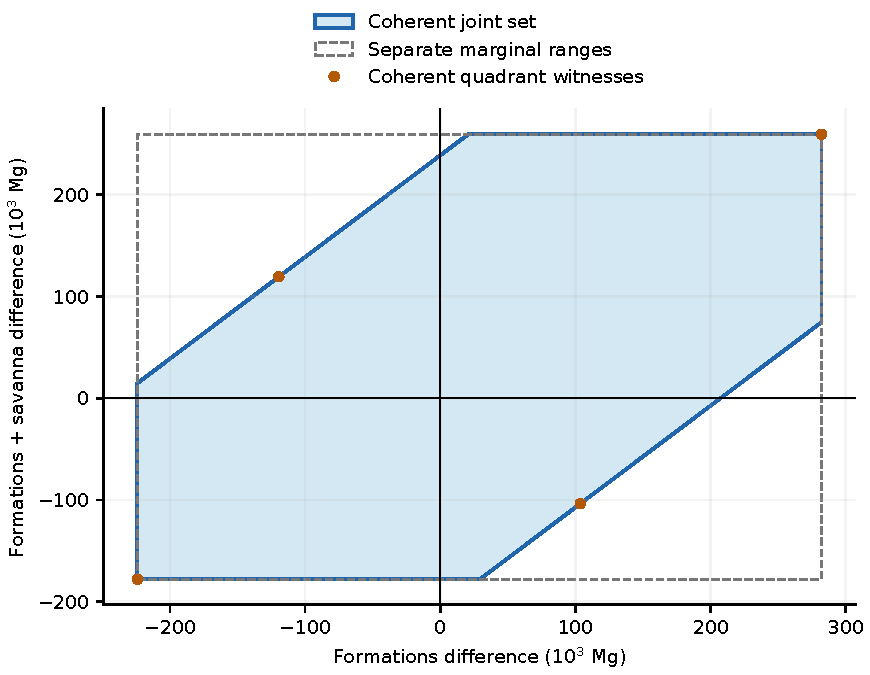
\includegraphics[width=.78\textwidth]{joint_identification_F11.pdf}
\caption{Sharp joint difference set for the nested mapped groups, conditional on exact point maps, nonnegative unrestricted allocation and no temporal coupling. The added-savanna constraint cuts off combinations admitted by the rectangle of marginal ranges. Four reconstructed allocations attain every strict sign quadrant while preserving all native-cell totals and component-presence geometry. Points are feasible allocation witnesses, not ecological observations or confidence regions.}\label{fig:joint}
\end{figure}



\subsection{Information increments and assumption-dependent signs}
The one-window information set has difference bounds $[-463.92,529.16]\times10^3$ Mg for either group, because both groups and their complements occupy positive area. Restoring native-cell mass observations narrows its width by $\ReductionForm\%$ for formations and $\ReductionSav\%$ for formations plus savanna (Supplementary Table~\SIref{tab:frontier}). Neither narrower set identifies a sign. The nine nested observation scales show that the width has already reached the one-window value at $32\times32$-cell blocks (Fig.~\ref{fig:identification}b). This is an exact comparison of identification sets under matched support, not a held-out reporting-rule or classification-performance comparison.

\paragraph{Restrictions required for a positive sign.}
Within the density-contrast sensitivity family, homogeneous allocation ($R=1$) gives positive model differences of $28.78\times10^3$ Mg for formations and $41.87\times10^3$ Mg for formations plus savanna. These are assumption-dependent outputs, not empirically identified forest-stock estimates. The lower difference bound reaches zero at $R=\RatioForm$ and $R=\RatioSav$, respectively (Fig.~\ref{fig:identification}c). Strict positive-sign identification within this family therefore requires a common contrast bound below the corresponding value; at the boundary zero is permitted. Neither contrast bound has been measured or validated here. The unrestricted sets remain the primary results. The sensitivity analysis identifies a specific additional information requirement rather than supplying it by assumption.

\begin{figure}[htbp]
\centering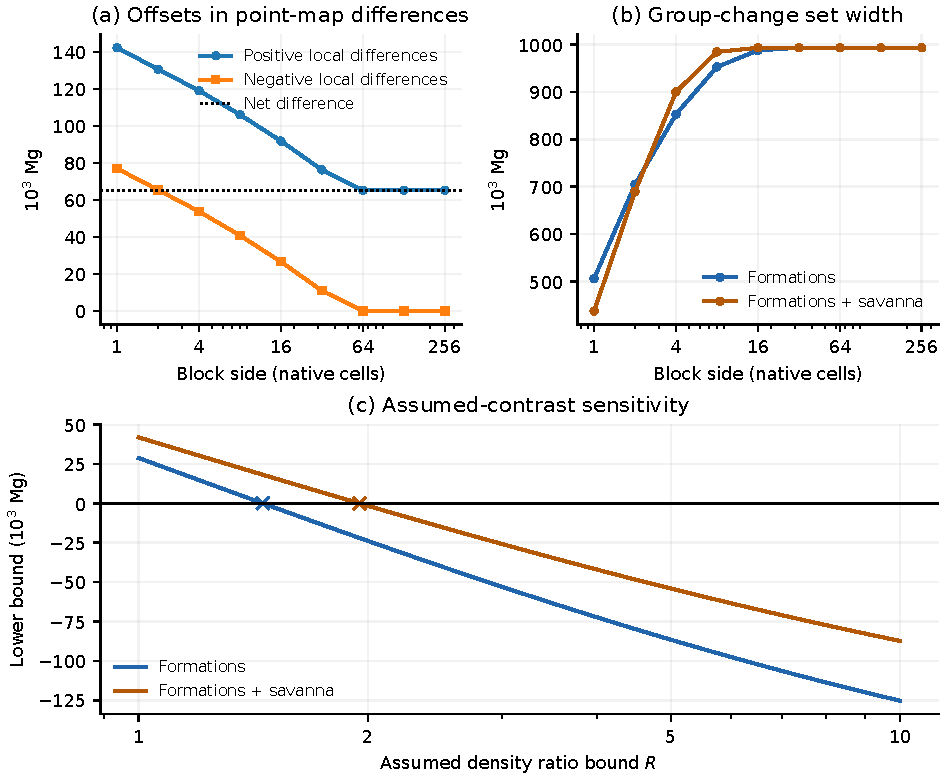
\includegraphics[width=\textwidth]{identification_frontier_F11.pdf}
\caption{Fixed-support point-map information analysis. (a) Summed positive and negative local mass differences decrease under spatial aggregation while the net is preserved. (b) Mapped-group difference-set widths increase as native-cell mass observations are replaced by block totals; cover definitions and footprint remain fixed. (c) The lower difference bound under an assumed within-cell density-contrast limit $R$; crosses mark zero-boundary values. No finite $R$ is empirically established. Native posting is not independent effective resolution. Panels describe conditional point-map arithmetic and allocation information, not calibrated ecological change, national trends or classification accuracy.}\label{fig:identification}
\end{figure}
\subsection{Unique mapped endpoint cohorts, not repeated annual events}\label{sec:flowresults}
Figure~\ref{fig:flows} summarizes all seven endpoint-cohort ranges. Brazilian formations have 22.711 million outflow hectare-events and 11.848 million inflow hectare-events during the eight annual transitions; Indonesia has 4.424 and 3.722 million, respectively. Event totals exceed net change and need not equal unique converted area.

The geographically restricted marked-flow networks imply Brazil formations-to-nonforest endpoint cohorts between 11.204 and 22.711 million ha; the corresponding cropland range is 0--7.014 million ha. Adding savannas changes those ranges to 18.374--35.847 and 0.009--8.662 million ha, respectively. Indonesian forest-to-nonforest is bounded by 1.312--4.424 million ha, forest-to-agriculture by 0.127--3.764 million ha, and forest-to-oil-palm by \textbf{0.112--2.326 million ha}. Each range includes its outward numerical allowance and conditions on the annual mapped capacities. Geographic restrictions tighten or preserve all raw bounds; all 634 saved primal/dual certificates satisfy the recorded residual criteria.

Direct annual forest-to-oil-palm transitions total 707,004 hectare-events, which is not the unique endpoint cohort bounded below (Supplementary Table~\SIref{tab:SI_transition_events}). The positive Indonesian oil-palm lower bound survives every aggregate-compatible intervening class path, but not arbitrary reference error. Its mapped minimum is 111,612 ha: retaining a positive reference-defined lower bound requires combined initial-forest and final-oil-palm class-set symmetric-difference error below that amount. No measured error budget meeting that condition is claimed. A small net-area error or pooled overall map accuracy does not supply it. Nor does this bound identify a biomass loss, direct clearing event, conversion association or causal effect.

\begin{figure}[htbp]
\centering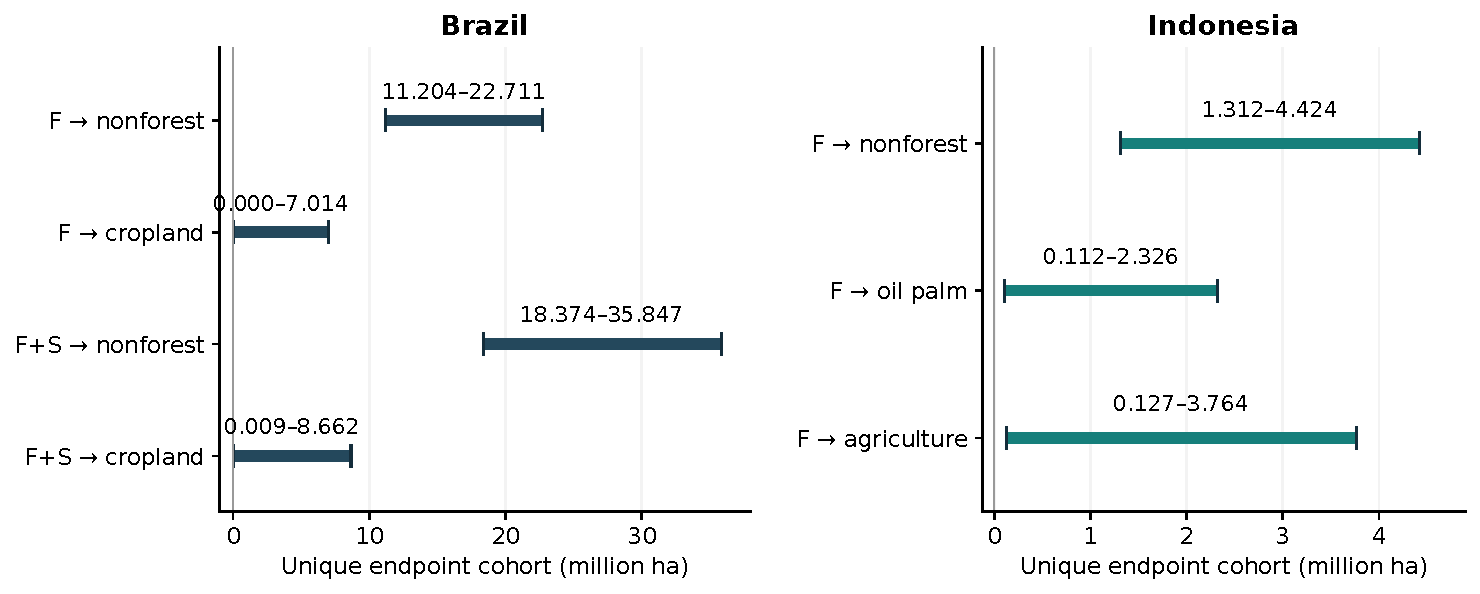
\includegraphics[width=1\textwidth]{endpoint_cohorts_F15.pdf}
\caption{Unique mapped 2015-forest-to-2023-destination cohort ranges under fine-geography transition capacities. Panels have different horizontal scales. F denotes each source forest/formation group; F+S adds Brazilian savannas. Numerical endpoints are in million ha; all include outward numerical allowances. These are feasible ranges, not confidence intervals, direct clearing events or calibrated ecological conversion. Supplementary Table~\SIref{tab:SI_conversion_exact} gives exact values.}\label{fig:flows}
\end{figure}
\subsection{Inventory evidence separates stock, period and uncertainty}\label{sec:inventoryresults}
Figure~\ref{fig:inventories} separates the inventory quantities, periods and uncertainty constructions. Finnish NFI12 and NFI13 growing-stock volumes are 2,475.192 and 2,551.964 million m$^3$, with reported standard errors 13.001 and 13.534 million m$^3$. Their difference is $+76.772$ million m$^3$ ($+3.10\%$). Equation~\ref{eq:invbonf}, with source rounding, gives an approximate 95\% sampling band of $[17.293,136.251]$ million m$^3$ without cross-cycle independence. The second-moment sensitivity is $[-41.896,195.440]$ million m$^3$, unresolved. A differential-bias budget of 17.293 million m$^3$ would exhaust the positive lower sampling bound; that budget is unmeasured. An unbounded differential systematic bias is not covered by either result. Total living-tree biomass is 1,744 versus 1,786 Mt including roots and stumps; the sum of stems plus branches/foliage is 1,350 versus 1,384 Mt. Neither receives the volume standard error or is promoted to the original AGB target.

French production-forest living volume is $2,716\pm45$ million m$^3$ in 2013--2017 and $2,916\pm47$ million m$^3$ in 2021--2025, where the published margins are 95\% endpoint halfwidths. The difference is $+200$ million m$^3$ ($+7.36\%$). A dependence-free band with at least 90\% sampling coverage, including full-unit rounding allowances, is $[104,296]$ million m$^3$. Under the additional marginal-normal interpretation, the approximate 95\% band is $[90.502,309.498]$ million m$^3$; four-endpoint simultaneous adjustment gives $[78.210,321.790]$ million m$^3$ for this longest contrast. These remain conditional on comparable measurement targets and methods, with differential bias $B$ widening either side. The shorter 2018--2022 and 2019--2023 comparisons against 2021--2025 are also retained: their approximate 95\% pairwise bands include zero. The latest overlapping windows must not be used as independent replicates, and none is an exact endpoint AGB comparison.

The Canadian inventory-domain annualized AGB change is $+17.639$ Mt/year with a provider-labelled halfwidth of 38.918 Mt/year, giving the unrounded reported range $[-21.279,56.557]$ Mt/year. The net direction is unresolved by that range. Subtype estimates concern contemporaneous class-defined stocks, not tracked biological cohorts; the complete component intervals are retained in Supplementary Table~\SIref{tab:SI_Canada_components}. The separate total relative standard error is labelled 1.16\%; applying the usual definition would imply a standard error of 0.205 Mt/year, irreconcilable with the 38.918 halfwidth under ordinary normal or large-sample $t$ conventions. The stock table does approximately reconcile, so the change export is not silently treated as the same statistical representation. We do not resolve the discrepancy by selecting the smaller uncertainty or assigning an unsupported confidence level. Projection, artificial-change filtering, geographic omissions and timing further prevent a primary national AGB inference.
\begin{figure}[htbp]
\centering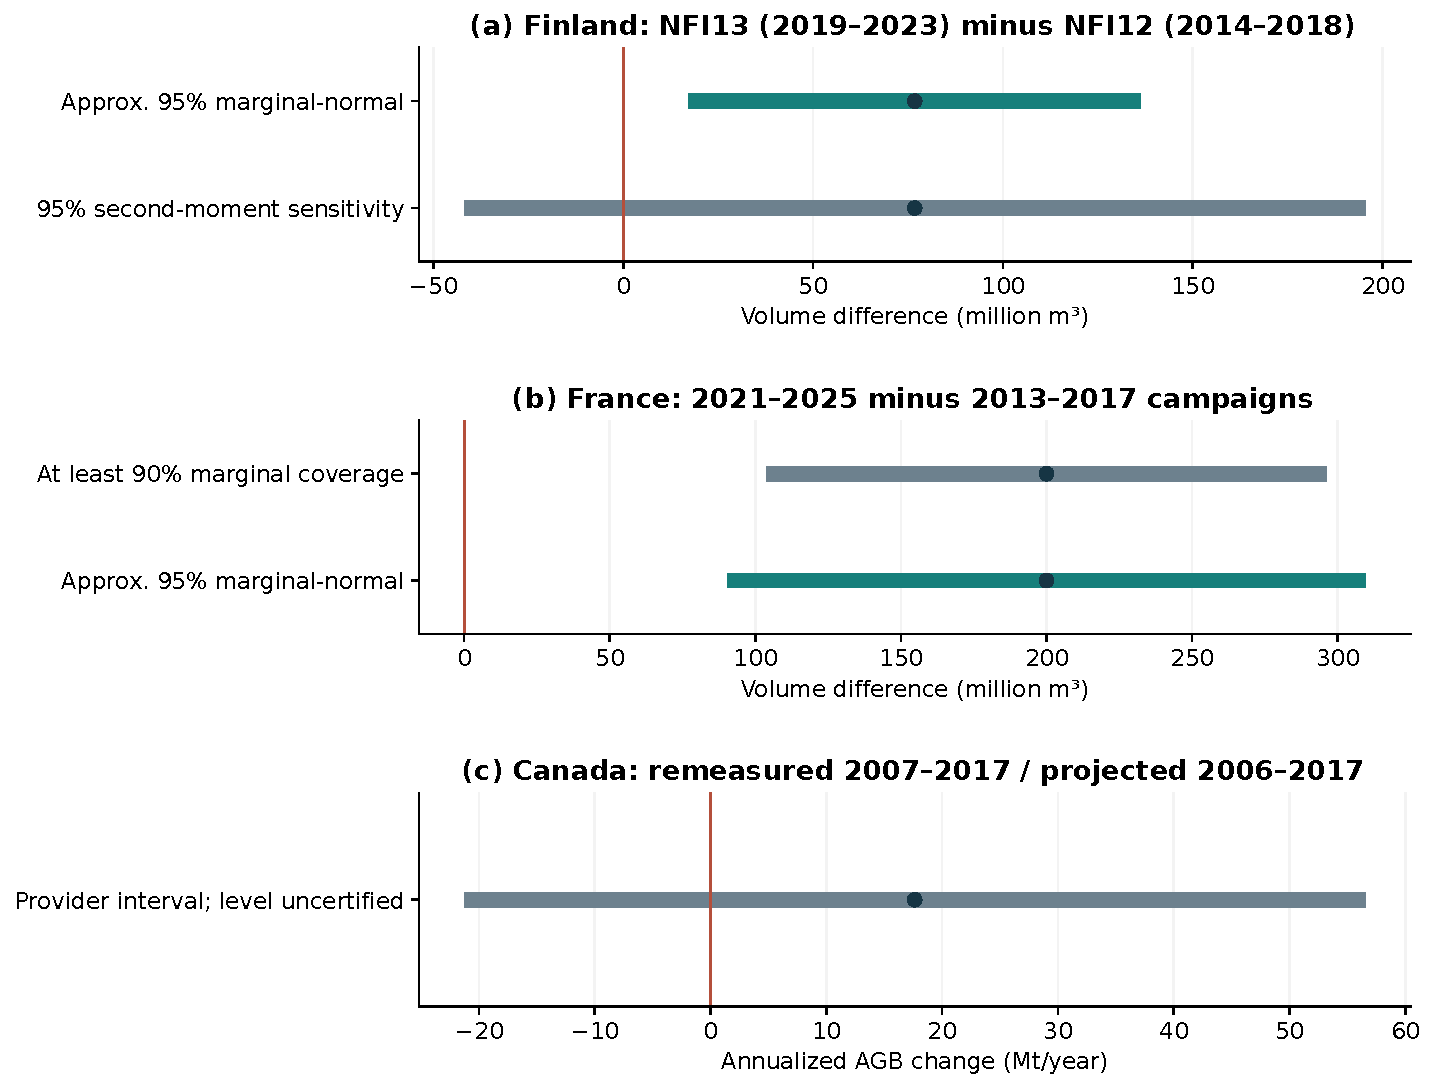
\includegraphics[width=1\textwidth]{inventory_uncertainty_F15.pdf}
\caption{Inventory evidence on distinct periods and domains, not a pooled comparison. (a) Finnish cycle-volume difference: the approximate marginal-normal 95\% sampling band is positive; a second-moment sensitivity includes zero. (b) French longest cycle contrast: direct marginal-interval subtraction gives at least 90\% sampling coverage; the separate approximate 95\% band assumes marginal normality. Both exclude unbounded differential method bias. (c) Canadian earlier-domain annualized AGB change: the provider-labelled interval includes zero; its confidence level is not independently certified. Canadian RSE, projection and northern-coverage issues remain explicit. Units and horizontal scales differ.}\label{fig:inventories}
\end{figure}
\paragraph{Scope of the national biomass comparison.}
None of the eight calibrated national 2015--2023 forest-AGB analyses is complete. Mapped extent is not forest biomass, pooled volume is not an annual AGB endpoint, and a regional or earlier-domain inventory is not a national target-period observation. Canada's omitted northern geography is not assigned zero biomass. French method comparability and Finnish biomass precision require evidence distinct from the reported volume intervals. Australia and Cameroon remain unexecuted physical modules, not demonstrated cases of permanent data unavailability. Completion is distinct from sign resolution: a valid calibrated comparison could include zero. The conditional results above are retained on their actual estimands rather than excluded or promoted to a different target.

\section{Discussion}
The account coverage supports a multi-country comparison, but availability alone does not establish matched physical support. The distinction is consequential where country definitions, forest masks, mapped observation domains or density denominators differ. Whole-cell biomass averages and forest-only means require different area multipliers. Applying the same multiplier to both would change the physical quantity being estimated.

Spatial compensation also requires measurement-specific interpretation. Opposing local net changes can occur within an increasing national total, but spatial error can produce the same pattern in point estimates. Cancellation must therefore be evaluated with spatial covariance, resolution and zero-change error models. A diagnostic evaluated against a target-derived quality class would measure agreement with that processing rule, rather than independently verified ecological change.

The evidence distinguishes arithmetic cancellation in delivered point maps, mapped-group non-identification, and ecological composition masking. The first is quantified on common support, and the second is established by constructive allocations with opposite signs. The third requires independently supported account--asset outcomes and is not demonstrated by either result. The matched-information comparison measures identification-set narrowing, not reporting-rule accuracy. Source-specific national mapped extent and conditional inventory-cycle stock results are now quantified, but calibrated national primary-period forest-AGB trends, independently supported account--asset divergence and conversion associations are not established. National inference requires territorial and mask reconciliation, independently justified change uncertainty, and coverage-sensitive treatment of missing or converted pixels. Soil, wetlands and fisheries involve different observation domains and are outside the present assessment.

The Brazilian example separates mapped forest formations, savannas and plantations rather than treating all woody vegetation as one invariant target. Temporal filters and gap filling can affect endpoint timing, while map-wide classification accuracy does not determine local or transition accuracy. The public older reference-point representations and the current Collection 11 assessment use different reference vintages; sample reuse, design weights, boundary exclusions and transition-specific interpretation require compatibility assessment before change validation. Different map publishers do not establish independent errors, particularly where auxiliary information or reference data may overlap.

The biomass observation operator imposes a further distinction. Even an exactly known forest fraction does not allocate total woody biomass between forest and other parts of a mixed pixel. A whole-territory woody-biomass stock is a different estimand from forest-only stock; neither should be relabelled as the other. Extent--density decomposition requires the stock and forest-area operands to describe the same support. Multiplying native density by mapped forest fraction identifies no forest-only biomass estimate without an allocation assumption; the homogeneous sensitivity endpoint supplies such an assumption, not independent evidence. The computed allocation sets quantify one part of the identification problem while conditioning on uncertain point maps; they do not supply a calibrated change-resolution rule. The contrast boundaries make an additional information requirement explicit: within this family, positive-sign identification requires a uniformly small enough density contrast in all mixed cells and at both endpoints. Independent measurements or defensible ecological constraints could test such a restriction, but neither increased map detail nor an assumed contrast substitutes for paired change validation.

The provider validation and the present identification limits address different questions. A held-out stock comparison can assess map agreement on its reference support without identifying forest-specific biomass inside a mixed cell or calibrating a paired 2015--2023 change on the present footprint. The described validation screening excludes plots deforested between inventory and map dates, and temporal harmonization uses growth assumptions; transferring its error characteristics to converted land requires evidence beyond agreement among retained forest observations \citep[pp.~13, 18--19]{PVIR2026}. Reference measurement error, geolocation and within-pixel sampling also contribute to map--reference discrepancies. Accordingly, neither RMSD nor a globally pooled bias pattern is adopted as a local change-error model, and the absence of such a model here is not a claim that the v7 stock product lacks validation.

National physical evidence should neither be erased by a primary-target hold nor promoted into a different estimand. Indonesia's improving total account and decreasing mapped forest are a concrete nominal discordance; Brazil and Congo retain decreasing accounts alongside their mapped declines. They do not constitute a representative sample or an independent reporting-accuracy evaluation. The oil-palm cohort bound adds information unavailable from annual event totals, but its transfer to ecological conversion requires class-set error control. The French longer inventory contrast also adds information unavailable from heavily overlapping recent cycles, while retrospective method bias remains explicit. Canadian direct-change reporting avoids an arbitrary endpoint-covariance assumption yet still requires scrutiny of projection, geography and inconsistent uncertainty representations.

A practical reporting sidecar should therefore show the aggregate account and its components, a separately defined physical extent or stock, its period and territory, an appropriate interval or feasible set, and conversion diagnostics distinguished from event counts. Improving information availability is not the same as demonstrating improved reporting accuracy. That latter claim needs independent physical outcomes on common cases. Nor can subnational units replicate a single national account change for an association test. The present analyses concern what the observations support; broader causal attribution requires a separate design.

\section{Conclusions}
Actual national accounts show both increases and decreases, with frequent offsets among components. Three executed national mapped-cover series, conditional unique endpoint-cohort bounds and official inventory-cycle quantities add substantive empirical evidence. Their definitions, geographic domains, time operators and uncertainty remain distinct. Finnish and French volume increases are conditional sampling results, not national exact-endpoint AGB validation; the Canadian reported total-change interval is unresolved. In the fixed Brazilian footprint, increasing whole-cell point-map biomass coexists with offsetting local differences and both signs of cover-group change under coherent nonnegative allocations. Native-cell information narrows those sets without resolving either sign, while density-contrast boundaries specify testable auxiliary-information requirements. All eight primary calibrated national 2015--2023 forest-AGB analyses remain incomplete; this is not a count of completed negative or inconclusive findings. The combined results establish observed account trajectories and specific gains and limits in physical identification, not measured national ecological composition masking. Compatible inventory designs, direct change estimates, reference-based marginal intervals and defensible dependence or bias bounds provide legitimate routes for the remaining ecological test.

\section*{Data and code availability}
Source datasets are cited in the text. National account trajectories, mapped extent series, marked-flow capacities and certificates, inventory source cells, uncertainty diagnostics and the integrated numerical workbook accompany the local identification results. The deposit identifies the immutable earlier numerical dependencies and their original source hashes. Supplementary Information provides source definitions, analytical derivations and exact supporting tables; machine-readable results and computational code are supplied in the deposit. Derived account-availability tables, source definitions, file hashes and computational methods are available at \url{https://github.com/MIKEAA2020/general-sustainability/tree/main/batch%209/agent%202/ecomod_empirical_followup/F15_A01}. NEFBA-derived tables and figures are distributed under CC BY-SA 4.0. Boundary inputs and boundary-derived data retain their separately documented source licences and attribution requirements. Conditional allocation summaries, topological intersection counts, matched-scale comparisons, aggregate witness certificates and density-contrast sensitivity results are also supplied; raw native-density arrays are not redistributed. MapBiomas-derived cover summaries identify Collection 11 and the processing used; the provider permits public use with source attribution. Raw country land-cover images, biomass files and provider technical reports are not redistributed.

\section*{Declaration of generative AI in scientific writing}
\href{http://Arena.ai}{Arena.ai} Agent Mode was used to assist with computational methods and literature review.

\begin{thebibliography}{99}
\bibitem[Abaee(2026)]{Abaee2026} Abaee, A. (2026). A rising biocapacity total can mask ecological-capital land drawdown: a two-land model. Manuscript. \url{https://github.com/MIKEAA2020/general-sustainability/tree/main/batch%209/agent%202/ecomod_c17}.
\bibitem[Mancini et al.(2017)]{Mancini2017} Mancini, M. S., Galli, A., Niccolucci, V., Lin, D., Hanscom, L., Wackernagel, M., Bastianoni, S., and Marchettini, N. (2017). Stocks and flows of natural capital: Implications for Ecological Footprint. \emph{Ecological Indicators}, 77, 123--128. \url{https://doi.org/10.1016/j.ecolind.2017.01.033}.
\bibitem[Maes et al.(2023)]{Maes2023} Maes, J., Bruz\'on, A. G., Barredo, J. I., Vallecillo, S., Vogt, P., Rivero, I. M., and Santos-Mart\'in, F. (2023). Accounting for forest condition in Europe based on an international statistical standard. \emph{Nature Communications}, 14, 3723. \url{https://doi.org/10.1038/s41467-023-39434-0}.
\bibitem[Olofsson et al.(2014)]{Olofsson2014} Olofsson, P., Foody, G. M., Herold, M., Stehman, S. V., Woodcock, C. E., and Wulder, M. A. (2014). Good practices for estimating area and assessing accuracy of land change. \emph{Remote Sensing of Environment}, 148, 42--57. \url{https://doi.org/10.1016/j.rse.2014.02.015}.
\bibitem[Lo et al.(2026)]{Lo2026} Lo, K., Basnet, N., Miller, E., Srikanthalingam, B., Foley, B., Van Berkum, J. L., Long, A. H., Toneva, P., Ermina, M., and Klinkenberg, C. (2026). \emph{National Ecological Footprint and Biocapacity Accounts, Edition 2026 (1961--2025): Results and metadata, version 1.0}. Footprint Data Foundation. \url{https://footprint.info.yorku.ca/data/}.
\bibitem[Santoro and Cartus(2026)]{SantoroCartus2026} Santoro, M., and Cartus, O. (2026). ESA Biomass Climate Change Initiative: Global datasets of forest above-ground biomass for 2005--2012 and 2015--2024, v7.0. CEDA. \url{https://doi.org/10.5285/6429d1aafe1e43b9b414e4a5a7f8b903}.
\bibitem[CCI Biomass(2026)]{PUG2026} CCI Biomass (2026). \emph{Product User Guide v7.0}. 19 March 2026. \url{https://climate.esa.int/en/projects/biomass/key-documents/}.
\bibitem[Runfola et al.(2020)]{Runfola2020} Runfola, D., et al. (2020). geoBoundaries: A global database of political administrative boundaries. \emph{PLOS ONE}, 15, e0231866. \url{https://doi.org/10.1371/journal.pone.0231866}. Country-specific geometry sources, represented years and commits: \url{https://www.geoboundaries.org/api.html}.
\bibitem[Copernicus Climate Change Service(2026)]{CDS2026} Copernicus Climate Change Service (2026). \emph{Land cover classification gridded maps from 1992 to present derived from satellite observations}. Catalogue and retrieval form accessed 29 October 2026. \url{https://doi.org/10.24381/cds.006f2c9a}.
\bibitem[MapBiomas Project(2026)]{MapBiomas2026} MapBiomas Project (2026). \emph{Collection 11 of the Annual Land Cover and Land Use Maps of Brazil}. General Algorithm Theoretical Basis Document, class codes and descriptions, and biome appendices. Accessed 29 October 2026. \url{https://brasil.mapbiomas.org/downloads/}.
\bibitem[CCI Biomass(2025a)]{ATBD2025} CCI Biomass (2025a). \emph{Algorithm Theoretical Basis Document, v7.0}. 17 December 2025. \url{https://climate.esa.int/media/documents/Algorithm_Theoretical_Basis_Document_ATBD_V7.0.pdf}.
\bibitem[CCI Biomass(2025b)]{E3UB2025} CCI Biomass (2025b). \emph{End to End ECV Uncertainty Budget, v7.0}. 17 December 2025. \url{https://climate.esa.int/documents/3354/End-to-End_ECV_Uncertainty_Budget_E3B_V7.0.pdf}.
\bibitem[CCI Biomass(2026b)]{PVIR2026} CCI Biomass (2026b). \emph{Product Validation and Intercomparison Report, v7.0}. 24 April 2026. \url{https://climate.esa.int/documents/3356/Product_Validation_Intercomparison_Report_PVIR_V7.0.pdf}.
\bibitem[Araza et al.(2026a)]{AGBref2026} Araza, A., Herold, M., Avitabile, V., et al. (2026a). AGBref: A global reference dataset of above-ground forest biomass. \emph{Research Square}, preprint, posted 9 January 2026. \url{https://doi.org/10.21203/rs.3.rs-8211898/v1}.
\bibitem[Araza et al.(2026b)]{AGBrefData2026} Araza, A., Bielig, C., and Flores, R. A. A. (2026b). AGBref---Global Reference Dataset for Above-Ground Biomass (AGB). Zenodo, record 20793072, file \texttt{agb-ref-v2.zip}. \url{https://doi.org/10.5281/zenodo.20793072}.

\bibitem[MapBiomas Indonesia(2026)]{MapBiomasIDN2026} MapBiomas Indonesia (2026). Collection 4.1 and Collection 3 land-cover statistics; Algorithm Theoretical Basis Document, Collection 4.1. \url{https://landy.mapbiomas.id/en/statistics}. \url{https://landy.mapbiomas.id/en/atbd}.
\bibitem[MapBiomas DR Congo(2026)]{MapBiomasCOD2026} MapBiomas Project (2026). Collection 1 of the Annual Land Use and Land Cover Maps of the Democratic Republic of the Congo, national statistics, legend and ATBD v1. \url{https://rdc.mapbiomas.org/telechargements/statistiques/}. \url{https://rdc.mapbiomas.org/telechargements/atbd/}.
\bibitem[Korhonen et al.(2021)]{Korhonen2021} Korhonen, K. T., Ahola, A., et al. (2021). Forests of Finland 2014--2018 and their development 1921--2018. \emph{Silva Fennica}, 55, article 10662. Supplementary S2, Table 20a. \url{https://doi.org/10.14214/sf.10662}.
\bibitem[Korhonen et al.(2024)]{Korhonen2024} Korhonen, K. T., et al. (2024). Forests of Finland 2019--2023 and their development 1921--2023. \emph{Silva Fennica}, 58, article 24045. Supplementary S2, Table 55. \url{https://doi.org/10.14214/sf.24045}.
\bibitem[IGN(2018)]{IGN2018} IGN (2018). \emph{Le m\'emento, inventaire forestier, \ edition 2018}, pp. 28--29; and \emph{M\'ethodologie 2013--2017}, pp. 5, 9, 16--17. \url{https://inventaire-forestier.ign.fr/IMG/pdf/181127_memento_2018_v4.pdf}. \url{https://inventaire-forestier.ign.fr/IMG/pdf/181011_methodologie.pdf}.
\bibitem[IGN(2026)]{IGN2026} IGN (2026). \emph{R\'esultats nationaux}, standard production-forest volume tables, campaigns 2021--2025, with retained 2018--2022 and 2019--2023 editions. \url{https://inventaire-forestier.ign.fr/spip.php?rubrique250}. Historical publications: \url{https://inventaire-forestier.ign.fr/spip/spip.php?article709=}.
\bibitem[Canada's NFI(2025)]{CanadaNFI2025} Canada's National Forest Inventory (2025). \emph{First remeasurement and forest change estimates}, version 3.1, November 2025, Tables 17.0 and 17C.0 and associated relative-standard-error and interval tables. \url{https://nfi.nfis.org/en/resources}. General estimation procedures v1.13: \url{https://nfi.nfis.org/en/estimation}.

\end{thebibliography}
\end{document}
